\documentclass[]{standalone}
\usepackage[dvipsnames]{xcolor}
\usepackage{tikz-network}
\begin{document}
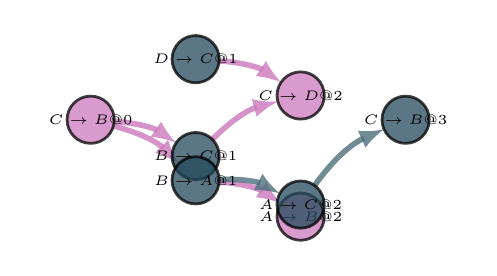
\begin{tikzpicture}
    \pgfmathsetmacro{\width}{4.0}
    \pgfmathsetmacro{\height}{2.0}
    \pgfmathsetmacro{\margin}{0.5 + 0.2}
    \tikzset{every node}=[font=\sffamily\bfseries]
    \clip (-\margin*\width cm,-\margin*\height cm) rectangle (\margin*\width cm,\margin*\height cm);
    \draw[draw,opacity=0] (-\margin*\width cm,-\margin*\height cm) rectangle (\margin*\width cm,\margin*\height cm);
    \Vertex[label=$C\to B@0$,fontsize=\fontsize{4}{10}\selectfont,RGB,color={204, 120, 188},size=0.6,opacity=0.75,style={draw opacity=0.75},x=-2.0,y=0.23076923076923084]{C->B@0};
\Vertex[label=$B\to C@1$,fontsize=\fontsize{4}{10}\selectfont,RGB,color={36, 74, 92},size=0.6,opacity=0.75,style={draw opacity=0.75},x=-0.6666666666666667,y=-0.23076923076923073]{B->C@1};
\Vertex[label=$B\to A@1$,fontsize=\fontsize{4}{10}\selectfont,RGB,color={36, 74, 92},size=0.6,opacity=0.75,style={draw opacity=0.75},x=-0.6666666666666667,y=-0.5384615384615384]{B->A@1};
\Vertex[label=$D\to C@1$,fontsize=\fontsize{4}{10}\selectfont,RGB,color={36, 74, 92},size=0.6,opacity=0.75,style={draw opacity=0.75},x=-0.6666666666666667,y=1.0]{D->C@1};
\Vertex[label=$A\to B@2$,fontsize=\fontsize{4}{10}\selectfont,RGB,color={204, 120, 188},size=0.6,opacity=0.75,style={draw opacity=0.75},x=0.6666666666666665,y=-1.0]{A->B@2};
\Vertex[label=$A\to C@2$,fontsize=\fontsize{4}{10}\selectfont,RGB,color={36, 74, 92},size=0.6,opacity=0.75,style={draw opacity=0.75},x=0.6666666666666665,y=-0.8461538461538461]{A->C@2};
\Vertex[label=$C\to D@2$,fontsize=\fontsize{4}{10}\selectfont,RGB,color={204, 120, 188},size=0.6,opacity=0.75,style={draw opacity=0.75},x=0.6666666666666665,y=0.5384615384615385]{C->D@2};
\Vertex[label=$C\to B@3$,fontsize=\fontsize{4}{10}\selectfont,RGB,color={36, 74, 92},size=0.6,opacity=0.75,style={draw opacity=0.75},x=2.0,y=0.23076923076923084]{C->B@3};
\Edge[bend=15,Direct,RGB,color={204, 120, 188},lw=2,opacity=0.8](C->B@0)(B->C@1);
\Edge[bend=15,Direct,RGB,color={204, 120, 188},lw=2,opacity=0.8](C->B@0)(B->A@1);
\Edge[bend=15,Direct,RGB,color={204, 120, 188},lw=2,opacity=0.8](B->C@1)(C->D@2);
\Edge[bend=15,Direct,RGB,color={204, 120, 188},lw=2,opacity=0.8](B->A@1)(A->B@2);
\Edge[bend=15,Direct,RGB,color={76, 112, 123},lw=2,opacity=0.8](B->A@1)(A->C@2);
\Edge[bend=15,Direct,RGB,color={204, 120, 188},lw=2,opacity=0.8](D->C@1)(C->D@2);
\Edge[bend=15,Direct,RGB,color={76, 112, 123},lw=2,opacity=0.8](A->C@2)(C->B@3);

\end{tikzpicture}
\end{document}
